\documentclass[parskip=full]{scrartcl}

\usepackage{amsmath}
\usepackage{hyperref}
\usepackage{graphicx}
\graphicspath {{images/}}
\hypersetup{
    colorlinks=true,
    citecolor=blue
}

\renewcommand\thesubsection{\thesection.\alph{subsection}}


\begin{document}


\title{CS698 - Assignment 3}
\subtitle{Winter 2017}
\author{
    Vineet John\\
    \texttt{v2john@uwaterloo.ca}
}
\date{\today}
\maketitle


\section{Gaussian Kernel Derivation} % (fold)
\label{sec:gaussian_kernel_derivation}



% section gaussian_kernel_derivation (end)


\section{Perceptron Learning Algorithm - Dual Formulation} % (fold)
\label{sec:perceptron_learning_algorithm_dual_formulation}



% section perceptron_learning_algorithm_dual_formulation (end)


\section{Non-linear Regression Techniques} % (fold)
\label{sec:non_linear_regression_techniques}

    \subsection{Regularized Generalized Linear Regression} % (fold)
    \label{sub:regularized_generalized_linear_regression}
    
        \begin{figure}[ht]
            \centering
            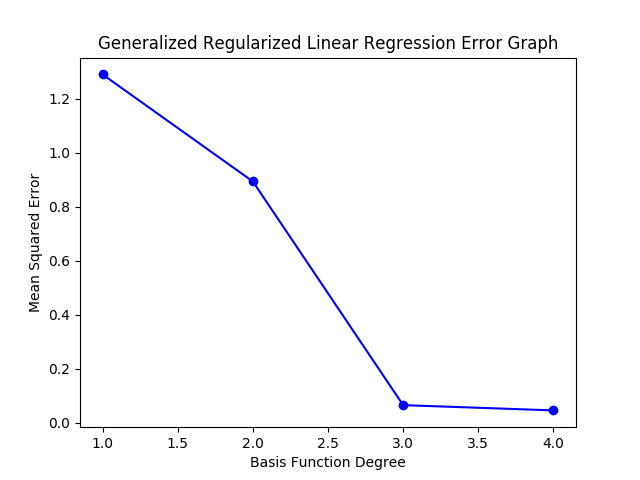
\includegraphics[width=0.6\textwidth]{3a_degree_vs_error.png}
            \caption{Regularized Generalized Linear Regression - Error vs Basis function degree}
            \label{fig:rglg_err_v_deg}
        \end{figure}

        \begin{figure}[ht]
            \centering
            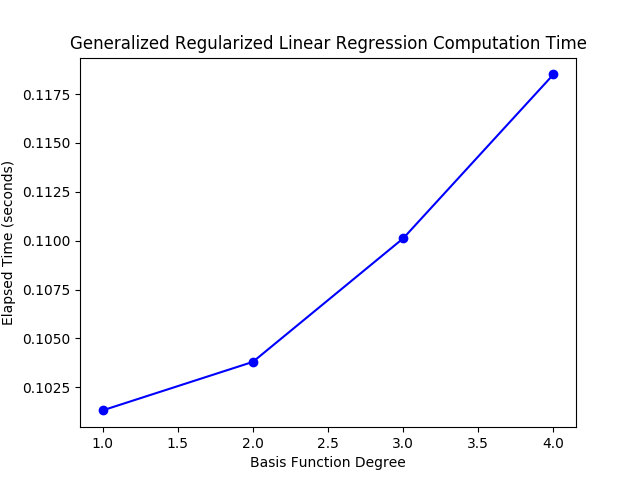
\includegraphics[width=0.6\textwidth]{3a_degree_vs_time.png}
            \caption{Regularized Generalized Linear Regression - Time vs Basis function degree}
            \label{fig:rglg_time_v_deg}
        \end{figure}

    % subsection regularized_generalized_linear_regression (end)

    \subsection{Bayesian Generalized Linear Regression} % (fold)
    \label{sub:bayesian_generalized_linear_regression}
    
        \begin{figure}[ht]
            \centering
            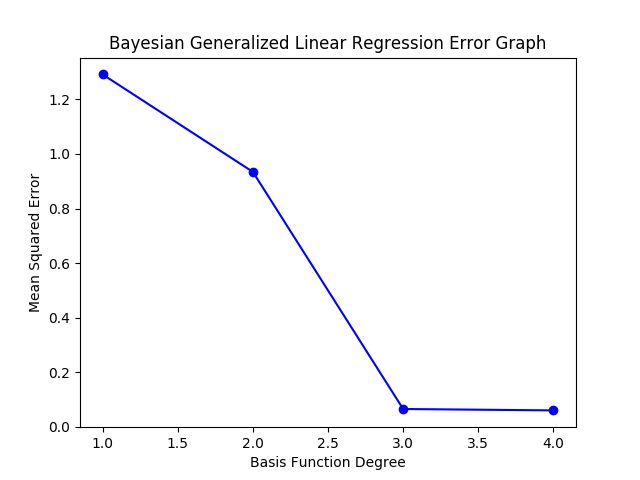
\includegraphics[width=0.6\textwidth]{3b_degree_vs_error.png}
            \caption{Bayesian Generalized Linear Regression - Error vs Basis function degree}
            \label{fig:bglg_err_v_deg}
        \end{figure}

        \begin{figure}[ht]
            \centering
            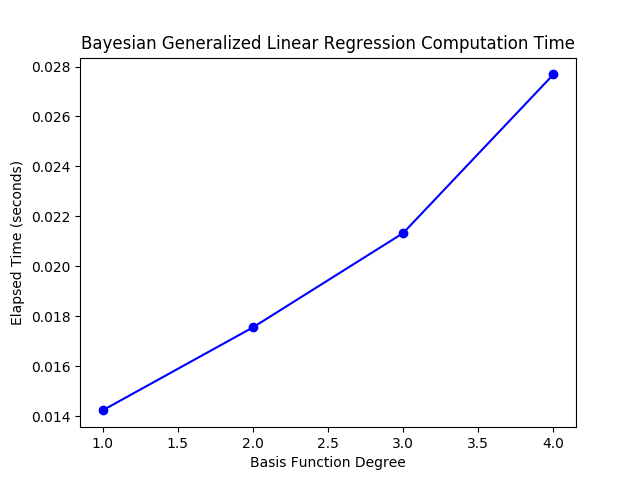
\includegraphics[width=0.6\textwidth]{3b_degree_vs_time.png}
            \caption{Bayesian Generalized Linear Regression - Time vs Basis function degree}
            \label{fig:bglg_time_v_deg}
        \end{figure}
    
    % subsection bayesian_generalized_linear_regression (end)

    \section{Gaussian Process Regression} % (fold)
    \label{sec:gaussian_process_regression}
    
    % section gaussian_process_regression (end)

% section non_linear_regression_techniques (end)


\end{document}
